\documentclass[9pt]{beamer}

% ============ Import Library ============
% Using vietnamese
\usepackage[utf8]{vietnam}
\usepackage[vietnam=nohyphenation]{hyphsubst}
\usepackage[vietnamese]{babel}
\usepackage[utf8]{inputenc}
% Some essential libs for math
\usepackage{amsmath, amsfonts, amssymb}
\usepackage{mathtools}
\usepackage{cases}
\usepackage{commath}
\usepackage{mathrsfs}
\usepackage{enumerate}
\usepackage[all]{xy}
% Essential libs for paper format
\usepackage{graphicx}
\usepackage{scrextend}
% Others
\usepackage{fancyhdr}
\usepackage[Glenn]{fncychap}
\usepackage{lipsum}
% \usepackage{tikz, tcolorbox}
\usepackage{amsthm}
% Font style
\setbeamertemplate{theorems}[numbered]

% ============ Configs ============
% Define commands
\renewcommand{\leq}{\leqslant}
\renewcommand{\geq}{\geqslant}
\newcommand{\nl}{\\[1.5mm]}
\newcommand{\nll}{\\[2.0mm]}
\newcommand{\nlll}{\\[3.0mm]}
\newcommand{\dlim}{\displaystyle\lim}
\newcommand{\N}{\mathbb N}
\newcommand{\Z}{\mathbb Z}
\newcommand{\Q}{\mathbb Q}
\newcommand{\R}{\mathbb R}
\newcommand{\C}{\mathbb C}
\renewcommand{\P}{\mathbb P}
\newcommand*{\QED}[1][$\square$]{%
\leavevmode\unskip\penalty9999 \hbox{}\nobreak\hfill
    \quad\hbox{#1}%
}
\newcommand*{\QEDFill}{\null\nobreak\hfill\ensuremath{\blacksquare}}
\newcommand{\startproof}{\noindent\textit{Chứng minh:\enskip}}

% Change largesymbols to other font
\DeclareMathOperator{\isom}{Isom}
\DeclareMathOperator{\im}{Im}
\DeclareMathOperator{\aut}{Aut}
\DeclareSymbolFont{largesymbols}  {OMX}{matha}{m}{n}

\theoremstyle{definition}
\newtheorem{remark}{Nhận xét}[section]
\newtheorem{define}{Định nghĩa}[section]
\newtheorem{proposition}{Mệnh đề}
\newtheorem{lemma1}{Bổ đề}
\newtheorem{theorem1}{Định lí}
\newtheorem{example1}{Ví dụ}
\newtheorem{corollary1}{Hệ quả}
\deftranslation[to=vietnamese]{theorem}{Định lí}
\deftranslation[to=vietnamese]{lemma}{Bổ đề}

% Beamer configs
\usetheme[progressbar=frametitle,block=fill]{metropolis}
\setbeamertemplate{frame numbering}[fraction]
\useoutertheme{metropolis}
\useinnertheme{metropolis}
\usefonttheme{metropolis}
\setbeamercolor{background canvas}{bg=white}

\definecolor{mycolor}{rgb}{0.75, 0.0, 0.0}
\usecolortheme[named=mycolor]{structure}
% title info
\date{}
\author{\textbf{SV trình bày:} Nguyễn Đình Đăng Khoa\\[2mm]\textbf{GV hướng dẫn:} Bùi Anh Tuấn}
\title[Short title]{\huge\textbf{Nhóm tinh thể}}
\subtitle{\normalsize{Báo cáo đề tài REU - VIASM}}
\setbeamersize{text margin left = 16pt, text margin right = 16pt}

\begin{document}
\begin{frame}
    \titlepage
\end{frame}

\begin{frame}{Mục lục}
    \tableofcontents
\end{frame}

\begin{frame}{Ý tưởng hình học}
    \section{Ý tưởng hình học}
\end{frame}

\begin{frame}{Ý tưởng hình học}
    Ý tưởng sơ khởi nhất của nhóm tinh thể đó là nghiên cứu các hình mẫu (pattern) trên mặt phẳng.

    \begin{figure}[ht]
        \centering
        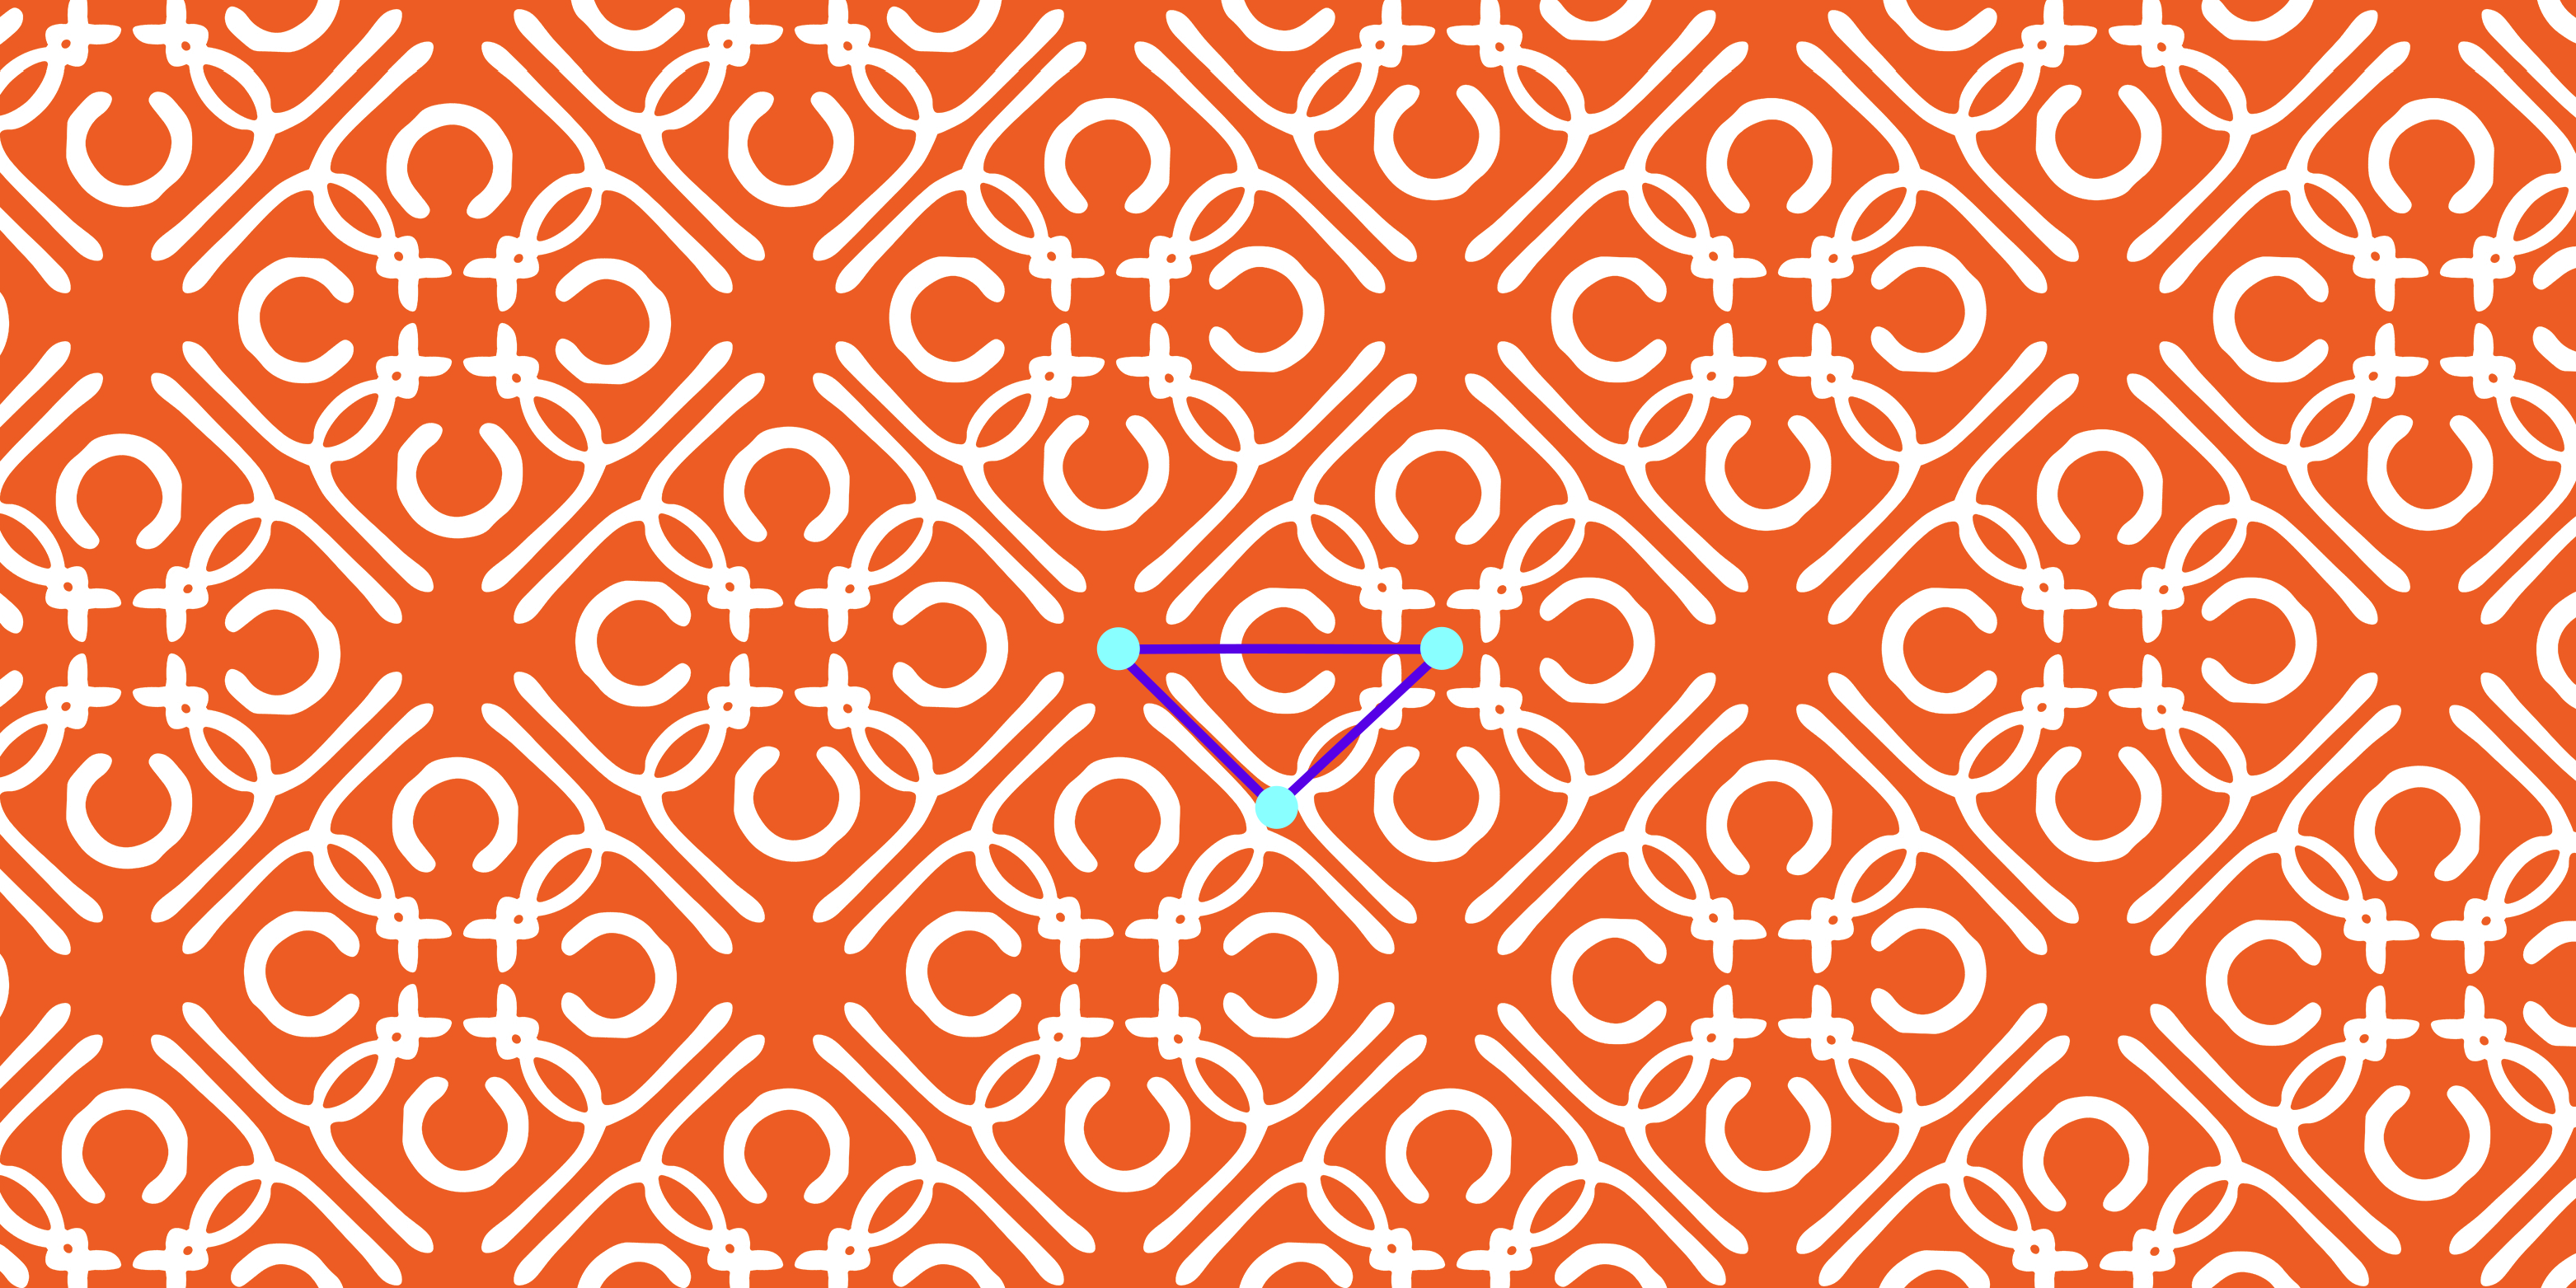
\includegraphics[scale=0.3]{assets/ngot-band-pattern.png}
        \caption{Hình mẫu được sử dụng trong album 3 của ban nhạc Ngọt.}
        \label{fig:ngot-album-pattern}
    \end{figure}
    Để ý hình mẫu trên được tạo ra bằng cách chọn trước một miền tam giác, sau đó bằng các phép biến đổi như tịnh tiến, xoay 45 độ, lật hình, ta có thể trải phủ miền đó ra khắp mặt phẳng và được hình mẫu như mong muốn.
\end{frame}

\begin{frame}{Ý tưởng hình học}
    Hơn nữa hình mẫu không bị phụ thuộc vào cách chọn trước miền tam giác mà chỉ phụ thuộc vào các phép biến đổi. Các phép biến đổi ấy mang cấu trúc nhóm và ta gọi nhóm đấy là nhóm hình nền (wallpaper group).
    \begin{figure}[ht]
        \centering
        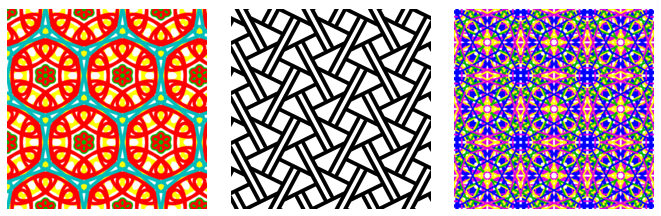
\includegraphics[scale=0.4]{assets/other-patterns.png}
        \caption{Các hình mẫu khác.}
        \label{fig:other-patterns}
    \end{figure}
\end{frame}

\begin{frame}{Ý tưởng hình học}
    Trong trường hợp 3 chiều, câu chuyện trở thành bài toán nghiên cứu cấu trúc tinh thể được hình thành bằng cách trải đều khối phân tử ra không gian.
    \begin{figure}[ht]
        \centering
        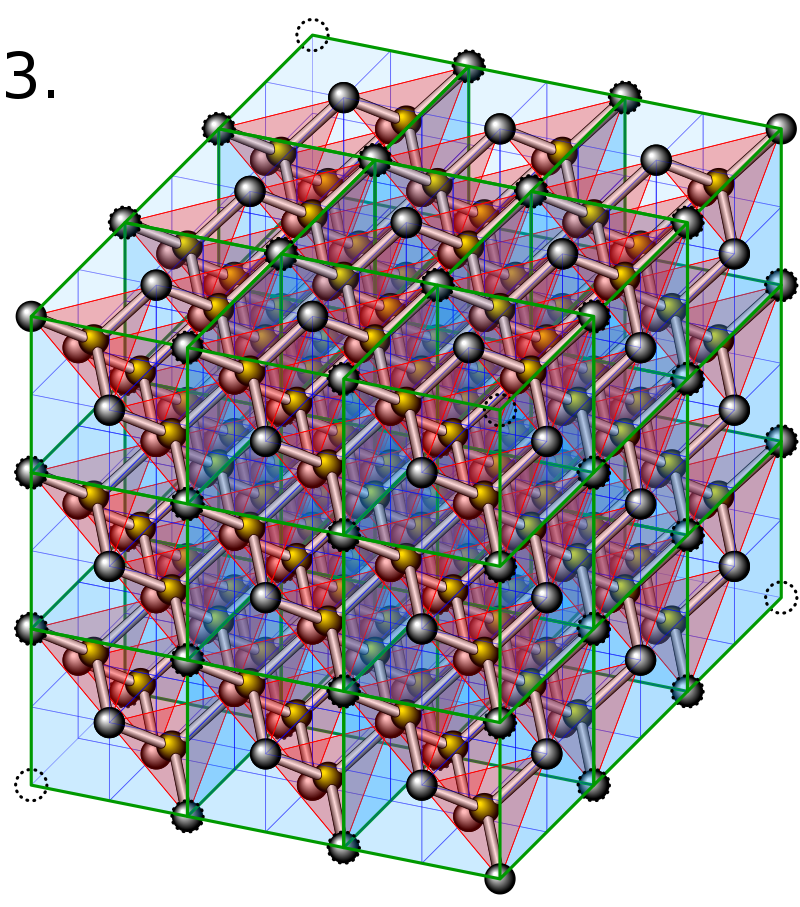
\includegraphics[scale=0.18]{assets/diamond-cube.png}
        \caption{Khối nguyên tử kim cương.}
        \label{fig:diamond-cube}
    \end{figure}
\end{frame}

\begin{frame}{Ý tưởng hình học}
    Không khó để ta tổng quát ý tưởng này lên $n$ chiều, và ta gọi chúng tổng quát là nhóm tinh thể. Cụ thể, một nhóm con $\Gamma$ của nhóm các phép đẳng cự $n$ chiều $E(n)$ được gọi là \alert{nhóm tinh thể} nếu thỏa hai tính chất sau:
    \begin{enumerate}[(i)]
        \item $\Gamma$ rời rạc trong $E(n)$.
        \item Tồn tại miền $D \subset \R^n$ compact sao cho $\Gamma D = \R^n$.
    \end{enumerate}
    Điều kiện (i) để đảm bảo các phép biến đổi trong $\Gamma$ không được xoay với góc nhỏ bất kì cũng như không được tịnh tiến với khoảng cách nhỏ tùy ý.
\end{frame}

\begin{frame}{Kiến thức chuẩn bị}
    \section{Kiến thức chuẩn bị}
\end{frame}

\begin{frame}{Kiến thức chuẩn bị - Không gian Euclid}
    \begin{center}
        \Large{\textbf{Không gian Euclid}}
    \end{center}

    Trong bài báo cáo này, ta coi $\R^n$ là không gian Euclid với tích vô hướng, chuẩn và metric lần lượt định nghĩa bởi
    $$
        \langle x,y \rangle = \sum_{i=1}^n x_i y_i,\enskip \|x\| = \sqrt{\langle x,y \rangle},\enskip d(x,y) = \|x-y\|
    $$
    với $x = (x_1,...,x_n), y = (y_1,...,y_n) \in \R^n$.
\end{frame}

\begin{frame}{Kiến thức chuẩn bị - Không gian Euclid}
    \begin{define}
        Cho $X$ và $Y$ là 2 không gian metric. Ánh xạ $f: X \rightarrow Y$ được gọi là một \alert{phép đẳng cự} nếu $f$ bảo toàn khoảng cách, nghĩa là với $a,b \in X$ thì
        $$
            d(a,b) = d(f(a),f(b)).
        $$
        Ta kí hiệu $\isom(X,Y)$ là tập các phép đẳng cự từ $X$ vào $Y$ và $\isom(X) := \isom(X,X)$.
    \end{define}
    \begin{proposition}
        $\isom(\R^n)$ có cấu trúc nhóm với phép toán là phép hợp nối ánh xạ. Hơn nữa ta gọi nhóm đó là \alert{nhóm Euclid $n$ chiều}, kí hiệu $E(n)$.
    \end{proposition}
\end{frame}

\begin{frame}{Kiến thức chuẩn bị - Không gian Euclid}
    \begin{define}
        Cho $a \in \R^n$. Ánh xạ $t_a: \R^n \rightarrow \R^n$ xác định bởi $t_a(x) = x + a$ được gọi là \alert{phép tịnh tiến} của $\R^n$.
    \end{define}
    \begin{proposition}
        Tập các phép tịnh tiến của $\R^n$ là nhóm con chuẩn tắc của $E(n)$. Ánh xạ $a \mapsto t_a$ xác định một đẳng cấu từ nhóm cộng $\R^n$ và nhóm các phép tịnh tiến của $\R^n$.
    \end{proposition}
    \startproof $A \circ t_a \circ A^{-1} (x) = A(A^{-1}x + a) = x + Aa = t_{Aa}(x)$.\qed

    Từ mệnh đề trên, ta đồng nhất $\R^n$ với nhóm các phép tịnh tiến của $\R^n$.
\end{frame}

\begin{frame}{Kiến thức chuẩn bị - Không gian Euclid}
    \begin{define}
        Ánh xạ tuyến tính $A: \R^n \rightarrow \R^n$ được gọi là \alert{trực giao} nếu với mỗi $x, y \in \R^n$,
        $$
            \langle x,y \rangle = \langle Ax, Ay \rangle.
        $$
    \end{define}
    \begin{proposition}\label{prop:orth_preserve_norm}
        Ánh xạ tuyến tính $A: \R^n \rightarrow \R^n$ trực giao khi và chỉ khi $A$ bảo toàn chuẩn, nghĩa là với mỗi $x \in \R^n,\ \|x\| = \|Ax\|$.
    \end{proposition}
    \startproof Nếu $A$ trực giao thì $\|x\| = \sqrt{\langle x,x \rangle} = \sqrt{\langle Ax,Ax \rangle} = \|Ax\|$. Ngược lại, ta có
    $$
        \|x+y\|^2 = \|A(x+y)\|^2 = \|x\|^2 + \|y\|^2 + 2 \langle Ax,Ay \rangle.
    $$
    Hơn nữa $\|x+y\|^2 = \|x\|^2 + \|y\|^2 + 2 \langle x,y \rangle$, suy ra $ \langle Ax,Ay \rangle = \|x+y\|$.\qed
    \begin{proposition}
        Tập các ánh xạ tuyến tính trực giao từ $\R^n \rightarrow \R^n$ tạo thành một nhóm, được gọi là \alert{nhóm trực giao}, kí hiệu $O(n)$.
    \end{proposition}
\end{frame}

\begin{frame}{Kiến thức chuẩn bị - Không gian Euclid}
    \begin{proposition}
        Mọi phép đẳng cự của $\R^n$ đều có biểu diễn duy nhất dưới dạng hợp nối của một phép tịnh tiến và một phép trực giao. Nói cách khác, với $f \in E(n)$, tồn tại duy nhất $A \in O(n)$ và $a \in \R^n$ sao cho $f = t_a \circ A$.
    \end{proposition}
    \startproof Xét $a = f(0)$ và $A = t_{-a} \circ f$ là một phép đẳng cự và $A(0) = 0$. Hơn nữa ta kiểm tra được $A$ là một ánh xạ tuyến tính, do đó theo Mệnh đề \ref{prop:orth_preserve_norm} thì $A$ trực giao.

    Giả sử $f = t_a \circ A = t_b \circ B$. Ta có $A = t_{-a} \circ t_b \circ B$. Mà $A$ phải cố định $0$ do đó $t_{-a} \circ t_b = Id$, nghĩa là $a = b$, dẫn tới $A = B$. Vậy $f = t_a \circ A$ là biểu diễn duy nhất.\qed
\end{frame}

\begin{frame}{Kiến thức chuẩn bị - Không gian Euclid}
    \begin{corollary1}
        $E(n) = O(n) \ltimes \R^n$, trong đó với $(A,a),(B,b) \in O(n) \ltimes \R^n$,
        $$
            (A,a)(B,b) = (AB,Ab+a).
        $$
    \end{corollary1}
    \begin{proposition}
        Xét \alert{nhóm affine} $A(n) = GL_n(\R) \ltimes \R^n$. Khi đó ta có các bao hàm thức sau
        $$
            E(n) \subset A(n) \subset GL_{n+1}(\R).
        $$
    \end{proposition}
    \startproof Bao hàm $E(n) \subset A(n)$ được suy ra từ định nghĩa. Với bao hàm thứ hai, ta đồng nhất $(A,a) \in A(n)$ với ma trận $\begin{bmatrix}A & a\\ 0 & 1\end{bmatrix} \in GL_{n+1}(\R)$.\qed
\end{frame}

\begin{frame}{Kiến thức chuẩn bị - Nhóm topo}
    \begin{center}
        \Large{\textbf{Nhóm topo}}
    \end{center}

    \begin{define}
        Cho $G$ là nhóm, đồng thời có cấu trúc topo với phép toán trên nhóm $\square\cdot\square: G \times G \rightarrow G$ và phép nghịch đảo $\square^{-1}: G \rightarrow G$ là các ánh xạ liên tục. Khi đó ta gọi $G$ là \alert{nhóm topo}.
    \end{define}

    \begin{define}
        Nhóm topo $G$ được gọi là \alert{tác động liên tục} lên không gian $X$ nếu tác động $\square \cdot \square: G \times X \rightarrow X,\ (g,x) \mapsto gx$ là ánh xạ liên tục.
    \end{define}

    \textbf{Ví dụ:} Nhóm ma trận $GL_n(\R)$ là nhóm topo nếu ta coi $GL_n(\R)$ là không gian con của không gian Euclid $\R^{n^2}$ và phép toán trên nhóm là phép nhân ma trận. Do đó $E(n)$ là nhóm topo con của $GL_{n+1}(\R)$, hơn nữa $E(n)$ tác động liên tục lên $\R^n$ theo nghĩa
    $$
        \begin{bmatrix}A & a\\ 0 & 1\end{bmatrix} \begin{bmatrix}v \\ 1\end{bmatrix} = \begin{bmatrix}Av + a \\ 1\end{bmatrix}.
    $$
\end{frame}

\begin{frame}{Kiến thức chuẩn bị - Nhóm topo}
    \begin{define}
        Không gian $X$ được gọi là rời rạc nếu tập một điểm $\{x\}$ là tập mở với mọi $x \in X$.
    \end{define}

    \begin{lemma1}
        Không gian metric $X$ rời rạc khi và chỉ khi mọi dãy $\{x_n\}$ hội tụ trong $X$ rồi sẽ trở thành dãy hằng, nghĩa là tồn tại $N \in \N$ đủ lớn sao cho $x_n = x_{n+1},\ \forall n \geq N$.
    \end{lemma1}
    \startproof $(\Rightarrow)$ Xét $x_n \rightarrow x \in X$. Do $\{x\}$ là tập mở nên tồn tại $N \in \N$ sao cho $x_n \in \{x\},\ \forall n \geq N$.\\
    $(\Leftarrow)$ Xét $x \in X$ và với mọi dãy $\{x_n\} \subset X\setminus\{x\}$. Do $\{x_n\}$ sẽ trở thành dãy hằng nên dãy hội tụ về giá trị $x_N \in X\setminus \{x\}$ nào đó. Vậy $X\setminus \{x\}$ đóng, hay $\{x\}$ mở.\qed
    \begin{define}
        Không gian quỹ đạo của tác động $G$ lên $X$ được định nghĩa là tập các $G$-quỹ đạo, $X/G = \{Gx\ |\ x \in X\}$ với topo sinh bởi ánh xạ thương $p: X \rightarrow X/G$, $x \mapsto Gx$.
    \end{define}
\end{frame}

\begin{frame}{Nhóm tinh thể}
    \section{Nhóm tinh thể}
\end{frame}

\begin{frame}{Nhóm tinh thể}
    \begin{define}
        Cho $\Gamma \leq E(n)$. Ta nói
        \begin{enumerate}[(i)]
            \item $\Gamma$ rời rạc nếu $\Gamma$ rời rạc trong không gian Euclid $\R^{(n+1)^2}$.
            \item $\Gamma$ đối compact nếu $E(n)/\Gamma$ compact.
            \item $\Gamma$ tác động thật sự không liên tục lên $\R^n$ nếu với mỗi $x \in \R^n$, tồn tại lân cận $U_x$ sao cho $\{ \gamma \in \Gamma\ |\ \gamma U_x \cap U_x \neq \emptyset \}$ là tập hữu hạn.
            \item $\Gamma$ tác động tự do lên $\R^n$ nếu với mọi $x \in \R^n$, $\{ \gamma \in \Gamma\ |\ \gamma x = x\} = \{(I,0)\}$.
        \end{enumerate}
    \end{define}

    \begin{define}
        Nhóm tinh thể $n$ chiều là nhóm con rời rạc và đối compact của $E(n)$.
    \end{define}
\end{frame}

\begin{frame}{Nhóm tinh thể}
    Hai mệnh đề sau sẽ cho hàng loạt các định nghĩa tương đương cho nhóm tinh thể.
    \begin{proposition}\label{prop:discrete}
        Cho $\Gamma \leq E(n)$. Các mệnh đề sau tương đương
        \begin{enumerate}[(i)]
            \item $\Gamma$ rời rạc trong $E(n)$.
            \item $\forall x \in \R^n$, $\Gamma x$ rời rạc trong $\R^n$.
            \item $\Gamma$ tác động thật sự không liên tục lên $\R^n$.
        \end{enumerate}
    \end{proposition}

    \begin{proposition}\label{prop:cocompact}
        Cho $\Gamma \leq E(n)$. Khi đó các mệnh đề sau là tương đương
        \begin{enumerate}[(i)]
            \item $\Gamma$ đối compact.
            \item $\R^n/\Gamma$ compact.
            \item Tồn tại $D \subset \R^n$ compact sao cho $\Gamma D = \R^n$.
        \end{enumerate}
    \end{proposition}
\end{frame}

\begin{frame}{Nhóm tinh thể}
    \begin{define}
        Cho $X$ là không gian metric và $G \leq \isom{(X)}$. Tập mở liên thông $F \subset X$ được gọi là \alert{miền cơ bản} của $X$ nếu 
        $$
            X = \bigcup_{g \in G} g \bar{F}
        $$
        và $gF \cap g'F = \emptyset$ với $g \neq g' \in G$.
    \end{define}

    \textbf{Ví dụ:} Xét $A = \left(\begin{bmatrix}1 & 0 \\ 0 & -1\end{bmatrix}, \begin{bmatrix}1/2 \\ 0\end{bmatrix}\right)$ và $B = \left(I, \begin{bmatrix}0 \\ 1\end{bmatrix}\right) \in E(2)$. Khi đó $\Gamma = \langle A,B \rangle \leq E(2)$ là nhóm tinh thể, có miền cơ bản là $(0,1/2)\times(0,1)$ và không gian quỹ đạo $\R^2 / \Gamma$ là chai Klein.
\end{frame}

% \begin{frame}{Nhóm tinh thể}
%     \section{Định lí Bieberbach}
% \end{frame}

\begin{frame}{Nhóm tinh thể}
    \begin{theorem1}{\textbf{(Định lí Bieberbach)}}
        \begin{enumerate}
            \item Nếu $\Gamma \leq E(n)$ là nhóm tinh thể thì tập các phép tịnh tiến trong $\Gamma$, $\Gamma \cap (I \times \R^n)$ là nhóm abel tự do chuẩn tắc có hạng bằng $n$, và là nhóm abel tối đại có chỉ số hữu hạn.
            \item Hai nhóm tinh thể $n$ chiều đẳng cấu với nhau khi và chỉ khi chúng liên hợp với nhau trong $A(n)$.
            \item Với mỗi chiều $n \in \N$ thì chỉ có hữu hạn các nhóm tinh thể $n$ chiều.
        \end{enumerate}
    \end{theorem1}
    Định lí Bieberbach thứ 3 chính là câu trả lời cho câu hỏi thứ 18 của David Hilbert.
\end{frame}

\begin{frame}{Nhóm tinh thể}
    Định lí Bieberbach thứ nhất cho ta dãy khớp
    \begin{center}
        $\begin{array}{ccccc}
            & 1 && 1 \\ & \downarrow && \downarrow \\ {\text{normal subgroup} \atop \text{lattice of translations}} & \Z^n &\subset& \R^n & {\text{translation} \atop \text{group}} \\ & \big\downarrow && \big\downarrow \\ {\text{crystallographic} \atop \text{group}} & \Gamma &\subset& E(n) & {\text{Euclidean} \atop \text{isometry group}} \\ & \big\downarrow && \big\downarrow \\ {\text{point} \atop \text{group}} & G &\subset& O(n) & {\text{orthogonal} \atop \text{group}} \\ & \downarrow && \downarrow \\ & 1 && 1
        \end{array}$
    \end{center}
    Trong đó $G$ là nhóm hữu hạn.
\end{frame}

\begin{frame}{Nhóm tinh thể}
    \begin{theorem1}{\textbf{(Định lí Zassenhaus)}}

        Một nhóm $\Gamma$ bất kì đẳng cấu với nhóm tinh thể $n$ chiều khi và chỉ khi $\Gamma$ có nhóm con abel tự do chuẩn tắc với hạng bằng n, hơn nữa là nhóm con abel tối đại trong $\Gamma$ và có chỉ số hữu hạn.
    \end{theorem1}
    Định lí trên đưa cho ta phương pháp phân loại nhóm tinh thể $n$ chiều dựa trên lý thuyết nhóm thuần thúy.
\end{frame}

\begin{frame}{Sử dụng đối đồng điều của nhóm để phân loại nhóm tinh thể}
    \section{Sử dụng đối đồng điều của nhóm để phân loại nhóm tinh thể}
\end{frame}

\begin{frame}{Sử dụng đối đồng điều của nhóm để phân loại nhóm tinh thể}
    \begin{center}
        \Large{\textbf{Đối đồng điều của nhóm}}
    \end{center}

    \begin{define}
        Cho $G$ là nhóm hữu hạn và $M$ là một $\Z G$-module. Với $n > 0$, ta đặt
        $$
            C^n(G,M) = \{ f: G^n \rightarrow M\ |\ f(g_1,...,g_n) = 0 \text{ Nếu } \exists g_i = 1 \}
        $$
        là tập các \alert{đối dây chuyền $n$ chiều}. Quy ước $C^0(G,M) = M$ và $C^n(G,M) = 0$ với $n < 0$. Từ đó ta định nghĩa toán tử đối biên $\delta^n: C^n(G,M) \rightarrow C^{n+1}(G,M)$ xác định bởi
        \begin{align*}
            (\delta^n f)(g_1,...,g_n) = &g_0f(g_1,...,g_n)\\
            +&\sum_{j=1}^n (-1)^j f(g_0,...,g_{j-2},g_{j-1}g_j,g_{j+1},...,g_n)\\
            +& (-1)^{n+1} f(g_0,...,g_{n-1})
        \end{align*}
        với $n > 1$. $(\delta^0 m)(g_1) = g_1 m - m$ và $\delta^n = 0$ với $n < 0$.
    \end{define}
\end{frame}

\begin{frame}{Sử dụng đối đồng điều của nhóm để phân loại nhóm tinh thể}
    \begin{proposition}
        $(C^n(G,M), \delta^n)_{n \in \Z}$ là một đối phức dây chuyền, nghĩa là $\delta^{n} \delta^{n-1} = 0$ với mọi $n \in \Z$. Từ đó ta định nghĩa
        \begin{itemize}
            \item $Z^n(G,M) := \ker \delta^n$ là tập các \alert{đối chu trình $n$ chiều}.
            \item $B^n(G,M) := \im\delta^{n-1}$ là tập các \alert{đối biên $n$ chiều}.
            \item $H^n(G,M) := Z^n(G,M) / B^n(G,M)$ là \alert{nhóm đối đồng điều thứ $n$} của $G$ với hệ số trong $M$.
        \end{itemize}
    \end{proposition}
\end{frame}

\begin{frame}{Sử dụng đối đồng điều của nhóm để phân loại nhóm tinh thể}
    \begin{center}
        \Large{\textbf{Phân loại nhóm tinh thể}}
    \end{center}
    Cho $\Gamma$ là nhóm tinh thể $n$ chiều và xét dãy khớp ngắn tương ứng
    \begin{equation}\label{eq:exact}
        \xymatrix{
            1 \ar[r] & \Z^n \ar[r]^-{i} & \Gamma \ar[r]^-{p} & G \ar[r] & 1
        }
    \end{equation}
    Khi đó $G$ tác động lên $\Z^n$ cho bởi biểu diễn 
    $$
        h_{\Gamma}: G \rightarrow \aut(\Z^n) \cong GL_n(\Z)
    $$
    $h_{\Gamma}(g)(e_i) = \bar{g} e_i \bar{g}^{-1}$, với $e_i \in \Z^n$ là cơ sở chuẩn tắc và $p(\bar{g}) = g$ với $\bar{g} \in \Gamma$. Hơn nữa, do tính abel tối đại của $\Z^n$ nên dẫn đến tác động này trung thành (nghĩa là $h_{\Gamma}$ đơn cấu).

    \textbf{Ý tưởng:} Thay vì phân loại trực tiếp dựa trên sự đẳng cấu giữa hai nhóm tinh thể, thì ta cố gắng phân loại các tác động của $G$ lên $\Z^n$. Thật vậy, ta sẽ chứng tỏ có sự tương ứng giữa nhóm tinh thể $n$ chiều với phần tử trong $H^1(G, \R^n / \Z^n)$.
\end{frame}

\begin{frame}{Sử dụng đối đồng điều của nhóm để phân loại nhóm tinh thể}
    $$
    \xymatrix{
        1 \ar[r] & \Z^n \ar[r]^-{i} & \Gamma \ar[r]^-{p} & G \ar[r] & 1
    }
    $$
    Để ý mặc dù ta có $E(n) = O(n) \ltimes \R^n$, nhưng chưa chắc $\Gamma = G \ltimes \Z^n$. Thật vậy, để điều đó xảy ra thì dãy trên phải chẻ, nghĩa là tồn tại $\tau: G \rightarrow \Gamma$ sao cho $p \circ \tau = id_{G}$. Do $p$ là ánh xạ chiếu lên $O(n)$ nên $\tau$ có dạng $\tau(g) = (g, \sigma(g))$ với $\sigma: G \rightarrow \R^n$. Ta gọi $\sigma$ là ánh xạ cắt.

    Cách chọn $\sigma$ là không duy nhất, do đó ta xét $s = p \circ \sigma: G \rightarrow \R^n / \Z^n$. Khi đó $s$ xác định duy nhất. Thật vậy giả sử tồn tại hai ánh xạ cắt $\sigma, \sigma'$. Khi đó
    $$
        (g, \sigma(g))(g, \sigma'(g))^{-1} = (g, \sigma(g))(g^{-1}, -g^{-1} \sigma'(h)) = (1, \sigma(g) - \sigma'(g)) \in \Gamma.
    $$
    Suy ra $\sigma(g) - \sigma'(g) \in \Z^n$, hay $p \circ \sigma' = p \circ \sigma'$.\qed
\end{frame}

\begin{frame}{Sử dụng đối đồng điều của nhóm để phân loại nhóm tinh thể}
    \begin{proposition}
        Ánh xạ $s$ trên thỏa mãn hai tính chất
        \begin{itemize}
            \item $s(1) = 0$.
            \item $s(g_1g_2) = s(g_1) + g_1s(g_2)$.
        \end{itemize}
    \end{proposition}

    \begin{corollary1}
        Tập các ánh xạ $s: G \rightarrow \R^n / \Z^n$ như trên chính là tập các đối chu trình 1 chiều, $Z^1(G, \R^n / \Z^n)$. 
    \end{corollary1}

    Tóm lại, mỗi nhóm tinh thể $\Gamma$ xác định một đối chu trình 1 chiều. Ngược lại, với mỗi $s \in Z^1(G, \R^n / \Z^n)$ ta có thể xây dựng ngược lại nhóm tinh thể $n$ chiều
    $$
        \Gamma = \{ (g, v) \in E(n)\ |\ g \in G, v \in s(g) \}.
    $$
    Vậy thay vì phân loại các nhóm tinh thể đẳng cấu với nhau, thì ta có thể đi phân loại các đối chu trình 1 chiều $s: G \rightarrow \R^n / \Z^n$.
\end{frame}

\begin{frame}{Sử dụng đối đồng điều của nhóm để phân loại nhóm tinh thể}
    Theo Định lí Bieberbach thứ 2, ta cần khảo sát tác động liên hợp của nhóm affine $A(n) = GL_n(\R) \ltimes \R^n$ lên nhóm tinh thể $n$ chiều, nhưng ta sẽ khảo sát trên phương diện đối chu trình 1 chiều.

    Xét phép tịnh tiến $(1,a) \in A(n)$ và $s$ là đối chu trình 1 chiều cho bởi ánh xạ cắt $\sigma: G \rightarrow \R^n$. Ta tính được
    \begin{align*}
        (1,a)(g, \sigma(g))(1,a)^{-1} &= (1,a)(g, \sigma(g))(1,-a)\\
        &= (g, a + \sigma(g))(1,-a)\\
        &= (g, a + \sigma(g) - ga).
    \end{align*}
    Lấy thương $\R^n \rightarrow \R^n / \Z^n$ ta được đối chu trình 1 chiều có dạng $b_a(g) = \overline{a} - g\overline{a}$, với $\overline{a} = a + \Z^n \in \R^n / \Z^n$.
    \begin{proposition}
        Tập các đối chu trình 1 chiều có dạng $b_a$ chính là tập các đối biên 1 chiều, $B^1(G, \R^n / \Z^n)$.
    \end{proposition}
\end{frame}

\begin{frame}{Sử dụng đối đồng điều của nhóm để phân loại nhóm tinh thể}
    Vậy nhóm đối đồng điều thứ nhất $H^1(G, \R^n / \Z^n) = Z^1(G,\R^n / \Z^n) / B^1(G, \R^n / \Z^n)$ giúp ta đồng nhất các nhóm tinh thể $n$ chiều, sai khác nhau bởi tác động liên hợp cho một phép tịnh tiến.

    Cuối cùng, xét $(h,0) \in A(n)$, $h \in GL_n(\R)$,
    $$
        (h,0)(g,\sigma(g))(h,0)^{-1} = (h,0)(g, \sigma(g))(h^{-1}, 0) = (hgh^{-1},h(\sigma(g))).
    $$
    Từ đó ta định nghĩa tác động $h \in GL_n(\R)$ lên $s \in Z^1(G, \R^n / \Z^n)$ cho bởi
    $$
        (h \cdot s)(g) = hs(h^{-1}gh).
    $$
    Nếu $h$ nằm trong chuẩn hóa tử $N_{\aut(\Z^n)}(G) = \{ h \in \aut(\Z^n)\ |\ hG = Gh\}$ thì ta có thể nói tác động liên hợp của $h$ lên $s$ chính là tác động của $h$ lên $s$ mà ta vừa định nghĩa.
\end{frame}

\begin{frame}{Sử dụng đối đồng điều của nhóm để phân loại nhóm tinh thể}
    \begin{theorem1}
        Có sự tương ứng 1-1 giữa lớp đẳng cấu các nhóm tinh thể $n$ chiều và quỹ đạo của $N_{\aut(\Z^n)}(G)$ tác động lên $H^1(G, \R^n / \Z^n)$.
    \end{theorem1}
    Từ đó ta đưa ra phương pháp phân loại nhóm tinh thể $n$ chiều như sau:
    \begin{enumerate}
        \item Xác định tất cả các nhóm điểm $G$ có thể xảy ra.
        \item Với mỗi $G$, xác định biểu diễn cho tập sinh của $G$ và tính $N_{\aut(\Z^n)}(G)$.
        \item Với mỗi biểu diễn, tính $H^1(G, \R^n / \Z^n)$.
        \item Xác định quỹ đạo của $N_{\aut(\Z^n)}(G)$ tác động lên $H^1(G, \R^n / \Z^n)$.
    \end{enumerate}
\end{frame}

\begin{frame}{Phân loại trên 2 chiều}
    \section{Phân loại trên 2 chiều}
\end{frame}

\begin{frame}{Phân loại trên 2 chiều}
    \begin{proposition}
        Mọi phần tử $h \in \aut(\Z^2)$ trực giao có cấp hữu hạn thì phải có cấp $1,2,3,4$ hay $6$.
    \end{proposition}
    \begin{proposition}
        Mọi nhóm con hữu hạn trong $GL_2(\R)$ hoặc là nhóm cyclic, hoặc là nhóm nhị diện.
    \end{proposition}
    Từ hai bổ đề trên, ta kết luận tất cả các nhóm điểm $G$ chỉ có thể trong các khả năng sau
    $$
        e, \Z_2, \Z_3, \Z_4, \Z_6, D_1, D_2, D_3, D_4, D_6.
    $$
\end{frame}

\begin{frame}{Phân loại trên 2 chiều}
    \begin{figure}[ht]
        \centering
        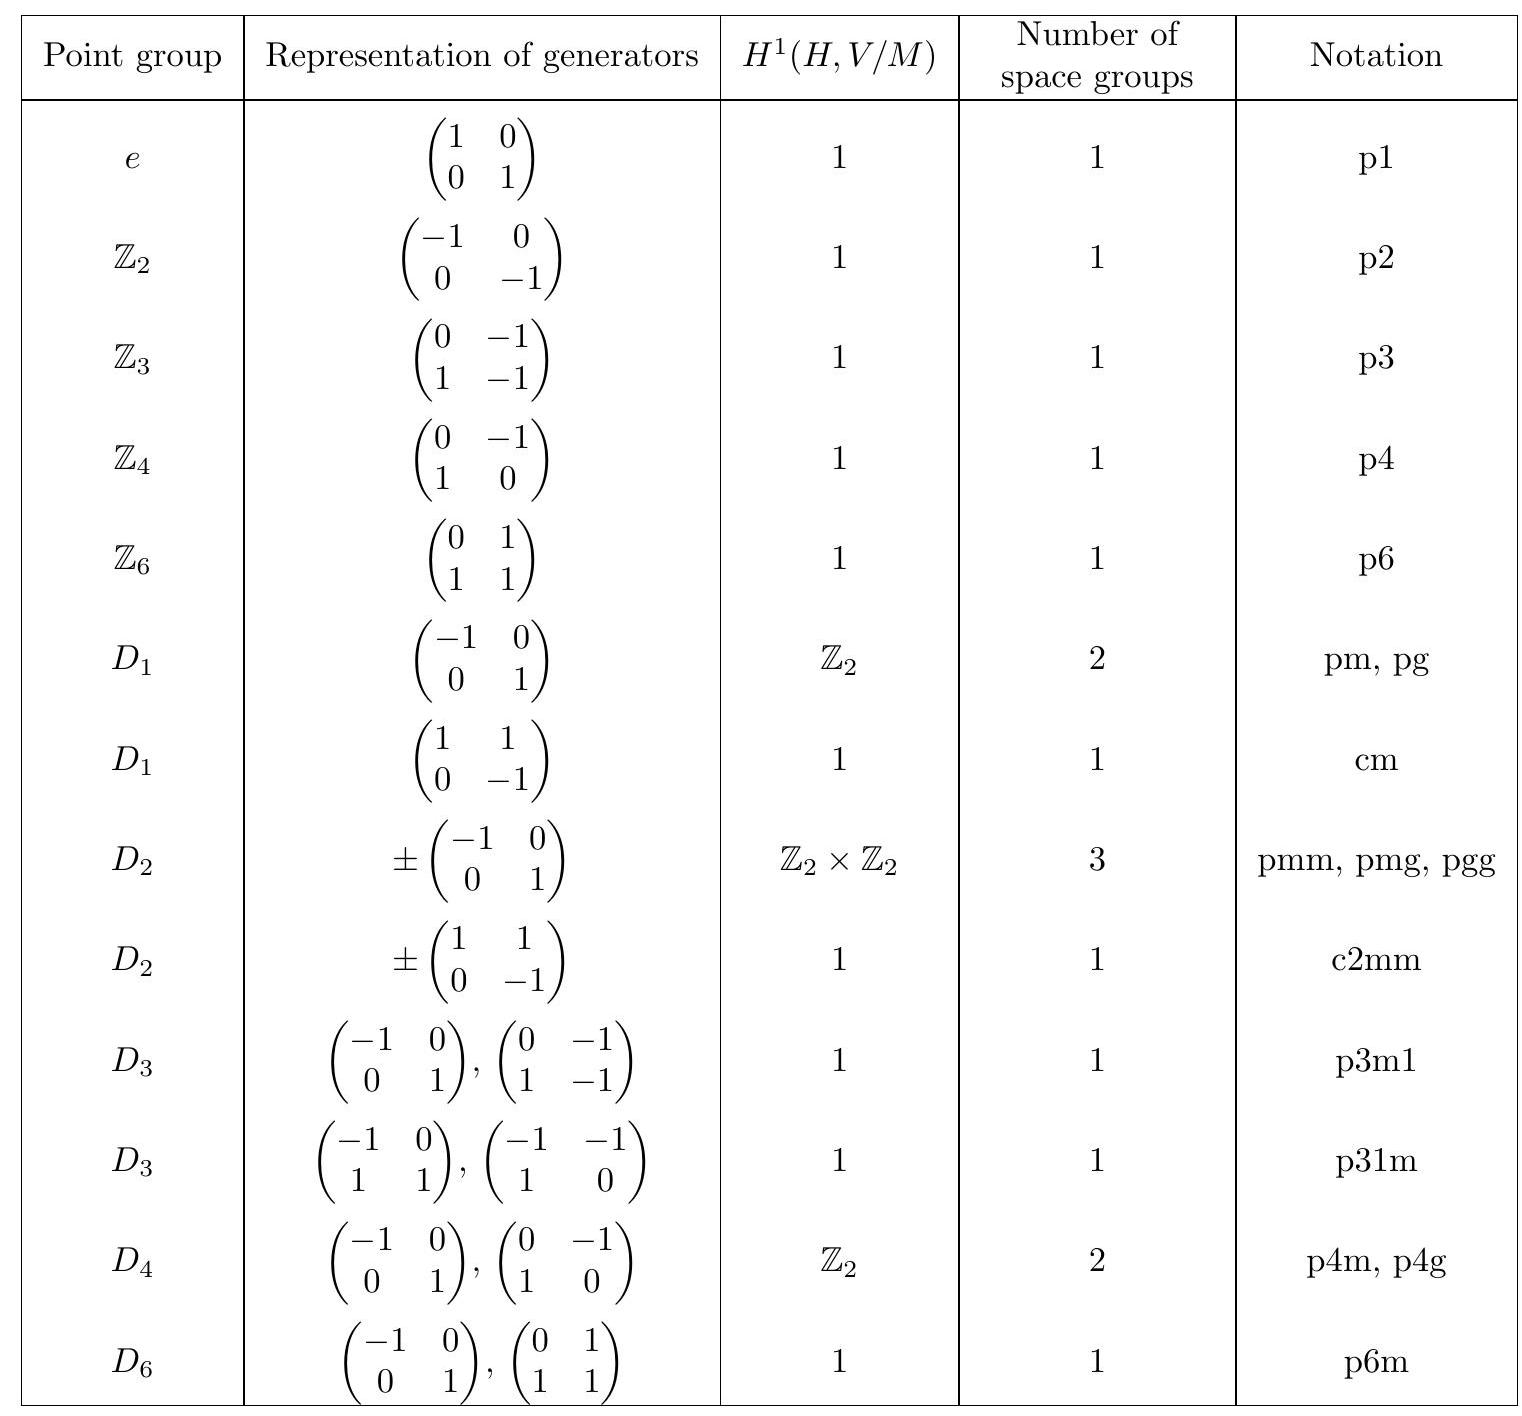
\includegraphics[scale=0.15]{assets/point-group-table.jpg}
        \caption{Bảng phân loại nhóm điểm 2 chiều.}
        \label{fig:point-group-table}
    \end{figure}
\end{frame}

\begin{frame}{Phân loại trên 2 chiều}
    \begin{center}
    \begin{tabular}{ |c|c| } 
        \hline
        $n$ & Số nhóm tinh thể $n$ chiều\\
        \hline
        1 & 2\\
        2 & 17\\
        3 & 219\\
        4 & 4783\\
        5 & 222018\\
        6 & 28927915\\
        \hline
    \end{tabular}
    \end{center}
    Schwarzenber chứng tỏ rằng, nếu ta gọi $s_n$ là số nhóm tinh thể $n$ chiều, thì tốc độ tăng của $s_n$ ít nhất phải tương đương với $2^{n^2}$.
\end{frame}
    
\begin{frame}{Tài liệu tham khảo}
    \renewcommand\refname{Tài liệu tham khảo}
\begin{thebibliography}{9}
    \bibitem{GeoCrys} Szczepański, Andrzej, \textit{Geometry of Crystallographic Groups}, WORLD SCIENTIFIC (2012).
    \bibitem{CrysCohom} Howard Hiller, \textit{Crystallography and Cohomology of Groups}, The American Mathematical Monthly (1986).
\end{thebibliography}

\end{frame}

\end{document}